%-----------------------------------------------------------------------
%
%   UFRJ  - Universidade Federal do Rio de Janeiro
%   COPPE - Coordena��o dos Programas de P�s-gradua��o em Engenharia
%   PEE   - Programa de Engenharia El�trica
%
%   COE-835  Controle adaptativo
%
%   Relat�rio da simula��o
%                                                         Ramon R. Costa
%                                                         05/out/09, Rio
%-----------------------------------------------------------------------
\documentclass[11pt,a4paper]{article}
\usepackage[latin1]{inputenc} %pacote para utilizar palavras acentuadas
\usepackage{amsmath,amssymb}  %pacotes do AMS
\usepackage{latexsym}         %pacote para incluir s�mbolos (ex.\Box)
\usepackage{fancybox,fancyhdr}%pacote com frescuras
\usepackage{graphicx}         %pacote para incluir figuras tipo eps
\usepackage[portuguese]{babel}
\usepackage{xcolor}
\usepackage{float} 
\usepackage{epstopdf}
\usepackage[inline]{enumitem}
\usepackage[a4paper]{hyperref}% Make sure it comes last of your loaded packages
\hypersetup{
  verbose,
  plainpages=false,
  bookmarks=true,
  colorlinks=true,
  linkcolor=blue
}
     
%----------------------------------------------------------------------
%
%   Macros utilizados no LATEX
%                                                       Ramon R. Costa
%                                                       13/out/17, Rio
%----------------------------------------------------------------------
\newcount\m
\newcount\n

\def\twodigits#1{\ifnum #1<10 0\fi \number#1}

\def\hours{\n=\time \divide\n 60
    \m=-\n \multiply\m 60 \advance\m \time
    \twodigits\n:\twodigits\m}

\def\hora{\hours}

\def\fim{
  \medskip
  \begin{center}
    \rule[1mm]{30mm}{0.14mm}$\diamond$\rule[1mm]{30mm}{0.14mm}
  \end{center}
}

%----------------------------------------------------------------------
% A4 paper size & margins
\setlength {\textheight}    {25cm}%
\setlength {\textwidth}     {17.5cm}%
\setlength {\parindent}     {0mm}%
\setlength {\parskip}       {1mm}%
\setlength {\topmargin}     {-14mm}%
\setlength {\oddsidemargin} {-6mm}%
\setlength {\evensidemargin}{-6mm}%
\setlength {\columnsep}     {6mm}%

%----------------------------------------------------------------------
\def\codigo{COE-835}
\def\disciplina{Controle adaptativo}
\def\periodo{3o. período/2017}
\def\professor{Ramon}

\newcommand{\BOX}[1]{
  \framebox{{\color{magenta}\rule[-3mm]{1mm}{9mm}} ~~$\displaystyle
  \begin{aligned} #1 \end{aligned}$~~}\pagestyle{plain}
}

\newcommand{\RED}[1]{\colorbox{white}{\textcolor{red}{#1}}}
%\newcommand{\WoR}[1]{\colorbox{red}{\textcolor{white}{#1}}}
\newcommand{\BLU}[1]{\colorbox{white}{\textcolor{blue}{#1}}}
\newcommand{\GRE}[1]{\colorbox{green}{\textcolor{black}{#1}}}
\newcommand{\HI}[1]{\colorbox{yellow}{\textcolor{black}{#1}}}  %% Highlithed text

\newcommand{\estrela}[1]{
  \def\TXT{\RED{$\bigstar$ }}
  \hspace*{5mm}\TXT \hfill
  \parbox[t]{ \textwidth - \widthof{\TXT} - 5mm}{#1}
  \par
}

\def\Ltwo{\mbox{${\mathcal L}_2$}}
\def\Linf{\mbox{${\mathcal L}_\infty$}}

\newcommand{\sign}{\mbox{sign}}

\newcommand{\equacao}[2]{
  \makebox[40mm][l]{#1 \dotfill}: \quad \parbox[t]{8cm}
	{\begin{equation} \displaystyle
  \begin{aligned}
    #2
  \end{aligned} \end{equation}} \\
}

\newcommand{\sref}[1]{Section~\ref{#1}}
\newcommand{\fref}[1]{Fig.~\ref{#1}}
\newcommand{\tref}[1]{Table~\ref{#1}}
\newcommand{\thref}[1]{Theorem~\ref{#1}}
\newcommand{\aref}[1]{Assumption~\ref{#1}}
\newcommand{\norm}[1]{\left\lVert#1\right\rVert}
%\renewcommand{\qedsymbol}{}
\newcommand{\rev}[1]{{\color{red}#1}}
%\newcommand{\mat}[1]{\begin{bmatrix}#1\end{bmatrix}}

\newtheorem{remark}{Remark}
\newtheorem{lemma}{Lema}

%----------------------------------------------------------------------


%Set normal paragraph spacing
\setlength\parindent{24pt}

\begin{document}
%---------------------------------------------------------------------
\pagestyle{fancy}%
\renewcommand{\headrulewidth}  {0.4pt}%
\renewcommand{\footrulewidth}  {0.4pt}%
\lhead{\bfseries{Relat�rio do Trabalho 3}}%
\chead{}%
\rhead{\bfseries\thepage}%
\lfoot{}%
\cfoot{}%
\rfoot{[\hours] \quad \today}%
%---------------------------------------------------------------------
\begin{center}
  \huge{COE-835  Controle  adaptativo}  \\[20mm]

  \Large{Simula��es do Trabalho 3} \\[20mm]
\end{center}

\textbf{Grupo:} \quad \parbox[t]{10cm}{
Guilherme Pires Sales de Carvalho \\[2mm]
Matheus Ferreira dos Reis \\[2mm]
Renan Salles de Freitas \\[10mm]
}

\textbf{Algoritmo:} \quad \HI{Identifica��o de par�metros}\\[2mm]

\bigskip%
Caso: \quad \parbox[t]{10cm}{
  $~n = 1, 2, 3$ \quad (ordem da planta) \\[2mm]
  $n^* = 1$ \quad (grau relativo) \\[2mm]
  $n_p = 2, 4, 6$ \quad (\# de par�metros) \\[15mm]
}

%---------------------------------------------------------------------
\tableofcontents
\newpage
%---------------------------------------------------------------------
%---------------------------------------------------------------------
\section{Resumo das equa��es do m�todo}

Abaixo, resumimos algumas das principais equa��es utilizadas no m�todo.

\vspace{20mm}

 \newpage
%---------------------------------------------------------------------
\section{Identifica��o de par�metros}

Identifica��o de par�metros � usar a cole��o de sinais dispon�veis do sistema,
baseado em algum crit�rio de otimalidade e informa��o da estrutura,
para produzir uma estimativa dos par�metros desconhecidos da planta.
Identifica��o adaptativa dos par�metros � um procedimento de estima��o din�mica que faz uso da atualiza��o
dos sinais do sistema para estimar os par�metros desconehcidos, atualizados
on-line. A identifica��o adaptativa de par�metros � crucial para o projeto de
controladores adaptativos, onde os par�metros de controle devem ser atualizados 
on-line ao mesmo tempo em que o sistema est� em opera��o.

Considere um sistema linear invariante no tempo descrito pela equa��o
diferencial (Eq. \ref{eq:planta}):
%
\begin{equation}
P(s)[y](t) = Z(s)[u](t),
\label{eq:planta}
\end{equation}
%
onde $y(t) \in \mathbb{R}$ e $u(t) \in \mathbb{R}$ s�o os sinais medidos de
sa�da e entrada do sistema e
%
\begin{gather}
P(s) = s^n + p_{n-1}s^{n-1}+\ldots + p_1s+p_0,\\
Z(s) = z_ms^m + z_{m-1}s^{m-1}+\ldots + z_1s+z_0
\label{eq:poly}
\end{gather}
%
s�o os polin�mios em $s$, $s$ sendo o operador de diferencial
$s[x](t)=\dot{x}(t)$; e $p_i, i = 0,1,\ldots,n-1$, $z_i, i=0,1,\ldots,m$ com
$n>m$, s�o os par�metros desconhecidos da planta.

Escolhe-se um polin�mio est�vel $\Lambda(s) = s^n+\lambda_{n-1}s^{n-1}+\ldots+\lambda_1s+\lambda_0$. Multiplicando ambos os
lados da equa��o \ref{eq:planta} pelo filtro $\frac{1}{\Lambda(s)}$, temos:
 
\begin{equation}
y(t) = \frac{Z(s)}{\Lambda(s)}[u](t)+\frac{\Lambda(s)-P(s)}{\Lambda(s)}[y](t).
\label{eq:filter_plant}
\end{equation}

Introduzindo o vetor de par�metros e regressor:

\begin{equation}
\theta* =
\left[z_0,z_1,\ldots,z_{m-1},z_m,\lambda_0-p_0,\lambda_1-p_1,\ldots,\lambda_{n-2}-p_{n-2},\lambda_{n-1}-p_{n-1}\right]^\intercal
\in \mathbb{R}^{n+m+1},
\label{eq:parameters}
\end{equation}

\begin{gather}
\phi(t) =
\left[\frac{1}{\Lambda(s)}[u](t),\frac{s}{\Lambda(s)}[u](t),\ldots,\frac{s^{m+1}}{\Lambda(s)}[u](t),\frac{s^{m}}{\Lambda(s)}[u](t),\right.
\\
\left.
\nonumber
\frac{1}{\Lambda(s)}[y](t),\frac{s}{\Lambda(s)}[y](t),\ldots,\frac{s^{n-2}}{\Lambda(s)}[y](t),\frac{s^{n-1}}{\Lambda(s)}[y](t)
\right]^\intercal \in \mathbb{R}^{n+m+1},
\label{eq:regressor}
\end{gather}

podemos expressar \ref{eq:filter_plant} como:

\begin{equation}
y(t) = \theta^{*\intercal}\phi(t).
\label{eq:thetaphi}
\end{equation}

A implementa��o do filtro � realizada pela constru��o de dois sistemas
din�micos, na realiza��o de estados:

\begin{gather}
\dot{\omega}_1(t) = A_\lambda\omega_1(t)+bu(t)\\
\dot{\omega}_2(t) = A_\lambda\omega_2(t)+by(t),
\label{eq:statespace}
\end{gather}

onde $\omega_1(t) \in \mathbb{R}^n$, $\omega_2(t) \in \mathbb{R}^n$ e

\begin{equation}
A_\lambda = 
\begin{bmatrix}
    0      & 1      & 0      & \dots  & 0      & 0      \\
    0      & 0      & 1      & 0      & \dots  & 0      \\
    \vdots & \vdots & \vdots & \vdots & \vdots & \vdots \\
    0      & 0      & \dots  & \dots  & 0      & 1      \\
    -\lambda_0 & -\lambda_1 & \dots & \dots & -\lambda_{n-2} & -\lambda_{n-1} 
\end{bmatrix}
, b =
\begin{bmatrix}
    0  \\
    \vdots  \\
    0 \\
    1 \\ 
\end{bmatrix}
\in \mathbb{R}^n
\label{eq:statespace}
\end{equation}

E o vetor regressor $\phi(t)$ pode ser escrito como:
\begin{gather}
\phi(t) = \left[
(C_m\omega_1(t))^\intercal,\omega_2^\intercal(t)\right]^\intercal,\\
C_m = \left[I_{m+1},0_{(m+1)\times(n-m-1)}\right] \in \mathbb{R}^{(m+1)\times
n}.
\end{gather} 

Onde, $I_{m+1}$ � a matriz identidade de dimens�o $(m+1)\times (m+1)$.
 
Considere $\theta(t)$ a estimativa dos par�metros $\theta^*$. O erro de
estima��o pode ser definido como:

\begin{equation}
\epsilon(t) = \theta^\intercal(t)\phi(t)-y(t) =
\tilde{\theta}^\intercal(t)\phi(t), t\geq t_0.
\end{equation}

Neste trabalho, ser�o considerados dois algoritmos para a atualiza��o
da estima��o dos par�metros ($\theta$): m�todo do gradiente normalizado e m�todo
\textit{least-square}.

O algoritmo do gradiente normalizado para atualiza��o da estima��o dos
par�metros corresponde escolher a derivada de $\theta(t)$ na dire��o do
gradiente descendente, minimizando a fun��o custo normalizada:

\begin{gather}
J(\theta) = \frac{\epsilon^2}{2m^2} =
\frac{\tilde{\theta}^\intercal \phi \phi^\intercal \tilde{\theta}}{2m^2},\\
m^2 = 1+\kappa \phi^\intercal (t) \phi
\end{gather}

Derivando-se a fun��o custo, obt�m-se a lei de adapta��o param�trica:

\begin{gather}
\dot{\theta}(t) = -\frac{\Gamma \phi(t) \epsilon (t)}{m^2(t)}, \theta(t_0) =
\theta_0, t\geq t_0,
\end{gather}

onde $\Gamma = \Gamma^\intercal > 0$ � uma matrix de ganhos. Vale observar que �
poss�vel provar por Lyapunov a estabilidade e converg�ncia de $\epsilon =
\theta^\intercal(t)\phi(t)-y(t)$ para zero. Por�m, esta condi��o n�o garante
$\tilde{\theta} = 0$, apenas garante a ortogonalidade entre os vetores dos
par�metros e regressor. A converg�ncia � garantida quando h� excita��o
persistente no sistema.

No caso do algoritmo \textit{least-square} normalizado, a atualiza��o
param�trica � dada pela equa��o:

\begin{gather}
\dot{\theta}(t) = -\frac{P(t) \phi(t) \epsilon (t)}{m^2(t)}, \theta(t_0) =
\theta_0, t\geq t_0,\\
\dot{P}(t) = -\frac{P(t) \phi(t) \phi^\intercal(t) P(t)}{m^2(t)}, P(t_0) = P_0 =
P_0^\intercal>0,t\geq t_0,\\
m^2(t) = 1+\kappa \phi^\intercal (t) P(t) \phi(t), \kappa > 0.
\end{gather}

\section{Implementa��o}

O trabalho consiste em identificar dinamicamente os par�metros do sistema para plantas de primeira, segunda e terceira ordem. Nesta se��o, iremos descrever a implementa��o em MATLAB dos algoritmos do gradiente normalizado e \textit{least-square} normalizado.

A primeira etapa da implementa��o � definir as condi��es iniciais, par�metros do sistema a serem identificados, fun��o de transfer�ncia da planta, filtro e sinal de entrada.

As condi��es iniciais do sistema s�o os valores para $y(0)$, $\theta_0$ e $P_0$, este �ltimo somente no caso do m�todo \textit{least-squares} normalizado. Consideremos uma planta est�vel de terceira ordem de forma a exemplificar com o sistema mais geral deste trabalho:
%
\begin{gather}
P(s) \, [y](t) = Z(s) \, [u](t) \, \\
\nonumber P(s) = (s+0.5)^3 = s^3 + 1.5 s^2 + 0.75s + 0.125 \, \\
\nonumber Z(s) = (s+0.3)^3 = s^2 + 0.6 s + 0.09 \, \\
\nonumber \overrightarrow{pz} =
\begin{bmatrix}
  z_2 & z_1 & z_0 & p_2 & p_1 & p_0
\end{bmatrix}
^\intercal=
\begin{bmatrix}
  1 & 0.6 & 0.09 & 1.5 & 0.75 & 0.125
\end{bmatrix}
^\intercal \, \\
\nonumber u(t) = r(t) = \mathrm{dc} + a_1 \, \mathrm{sin}(w_1 \, t) + a_2 \, \mathrm{sin}(w_2 \, t) + a_3 \, \mathrm{sin}(w_3 \, t) \,.
\end{gather}

O sinal de refer�ncia deve possuir pelo menos seis frequ�ncias para esse sistema, pois h� seis par�metros desconhecidos (Se��o 3.5 - Tao). Sendo assim, foi escolhido um sinal de refer�ncia com tr�s sen�ides de frequ�ncias distintas. Al�m disso, o sistema � dito com excita��o persistente se $u(t)$ n�o possui frequ�ncias do regressor $\phi(t)$. 
%
Agora, considere o seguinte filtro de terceira ordem:
%
\begin{gather}
\Lambda(s) = (s+1)^3 = s^3+3s^2+3s+1,\\
\nonumber \vec{\lambda} = 
\begin{bmatrix}
  \lambda_2 & \lambda_1 & \lambda_0
\end{bmatrix}
^\intercal=
\begin{bmatrix}
  3 & 3 & 1
\end{bmatrix}
^\intercal \,.
\end{gather}

O vetor de par�metros ideais � definido como:
%
\begin{gather}
\theta^* =
\begin{bmatrix}
  z_0 & z_1 & z_2 &(\lambda_0-p_0) & (\lambda_1-p_1) & (\lambda_{2}-p_{2})
\end{bmatrix}
^\intercal = \\
\nonumber \theta^* =
\begin{bmatrix}
  \textrm{flip}\left(\overrightarrow{pz}(1:3)\right)  & \textrm{flip}\left(\vec{\lambda}-\overrightarrow{pz}(4:6)\right)
\end{bmatrix}
^\intercal = \\
\nonumber \theta^* =
\begin{bmatrix}
  0.09 & 0.6 & 1 & 0.875 & 2.25 & 1.5
\end{bmatrix}
^\intercal \,.
\end{gather}

As equa��es do filtro $\frac{1}{\Lambda(s)}$ podem ser descritas como um sistema no espa�o de estados:
%
\begin{gather*}
\omega_1 = 
\begin{bmatrix}
  \omega_{11} & \omega_{12} & \omega_{13}
\end{bmatrix}
^\intercal \,, \\
%
\omega_2 = 
\begin{bmatrix}
  \omega_{21} & \omega_{22} & \omega_{23}
\end{bmatrix}
^\intercal \,,
\end{gather*}
%
\[
\begin{cases}
\dot{\omega}_{11} = \omega_{12}, \\
\dot{\omega}_{12} = \omega_{13}, \\
\dot{\omega}_{13} = u - \textrm{flip}(\vec{\lambda})^\intercal \, \omega_1
\end{cases}
\]

\[
\begin{cases}
\dot{\omega}_{21} = \omega_{22}, \\
\dot{\omega}_{22} = \omega_{23}, \\
\dot{\omega}_{23} = y - \textrm{flip}(\vec{\lambda})^\intercal \, \omega_2
\end{cases}
\]

Resumidamente:
%
\begin{gather}
\dot{\omega}_1 =
\begin{bmatrix}
  \omega_1(2:3) & y - \textrm{flip}(\vec{\lambda})^\intercal \omega_1
\end{bmatrix}
^\intercal,\\
%
\nonumber \dot{\omega}_2 =
\begin{bmatrix}
  \omega_2(2:3) & y - \textrm{flip}(\vec{\lambda})^\intercal \omega_2
\end{bmatrix}
^\intercal,\\
\phi = 
\begin{bmatrix}
  \omega_1 & \omega_2
\end{bmatrix}
\,.
\end{gather}

Podemos descrever a saída estimada e real do sistema pelos filtros:
%
\begin{gather}
y = \theta^{*\intercal} \, \phi \, \\
\hat{y} = \theta^\intercal \, \phi \, \\
\epsilon = \hat{y}-y = \tilde{\theta}^\intercal \, \phi \,.
\end{gather}

Finalmente, descrevemos a atualiza��o de $\theta$, os par�metros estimados,
conforme o gradiente normalizado ou pelo m�todo \textit{least-square}:
%
\[
\textrm{Gradiente Normalizado}
\begin{cases}
m^2 \leftarrow 1 + \phi^\intercal\phi\\
\dot{\theta} \leftarrow -\Gamma\ \phi \epsilon / m^2
\end{cases}
\]

\[
\textrm{Least-square Normalizado}
\begin{cases}
m^2 \leftarrow 1 + \phi^\intercal P\phi\\
\dot{\theta} \leftarrow -P \phi \epsilon / m^2\\
\dot{P} \leftarrow -P \phi \phi^\intercal P / m^2
\end{cases}
\]

Observe que no c�lculo de $m^2$, fixamos o valor do par�metro $\kappa$ em 1 para ambos os casos.

%---------------------------------------------------------------------
\section{Resultados das simula��es}

%Simula��o utilizando \HI{\texttt{Matlab/Simulink}}.

Nas simula��es, procuramos avaliar o comportamento do sistema para as seguintes condi��es:
%
\begin{enumerate*}[label=(\roman*)]
\item condi��o inicial $\theta(0)$;
\item sinal de refer�ncia $r(t)$;
\item ganho de adapta��o $\gamma$.
\end{enumerate*}

Apresentaremos os resultados obtidos atrav�s de simula��es no ambiente \HI{\texttt{Matlab/Simulink}} e os discutiremos na pr�xima se��o.

\subsection{Simula��o \#1}

Inicialmente, desejamos verificar o comportamento do sistema para varia��es no
sinal de refer�ncia $r(t)$ para podermos analisar a influ�ncia da persist�ncia
de excita��o.

%\bigskip%
%Par�metros e condi��es iniciais :
%
\begin{align*}
  y &= \frac{1}{s+2}u\,,  &  \Lambda &= \frac{1}{s+1}\,, & \theta(0) &= 0\,, \\
  \gamma &= 5\,, & r &= \HI{1, $1+5\textrm{sin}(t)$}\, \,.
\end{align*}

\bigskip%
\begin{figure}[H]
  \centering
  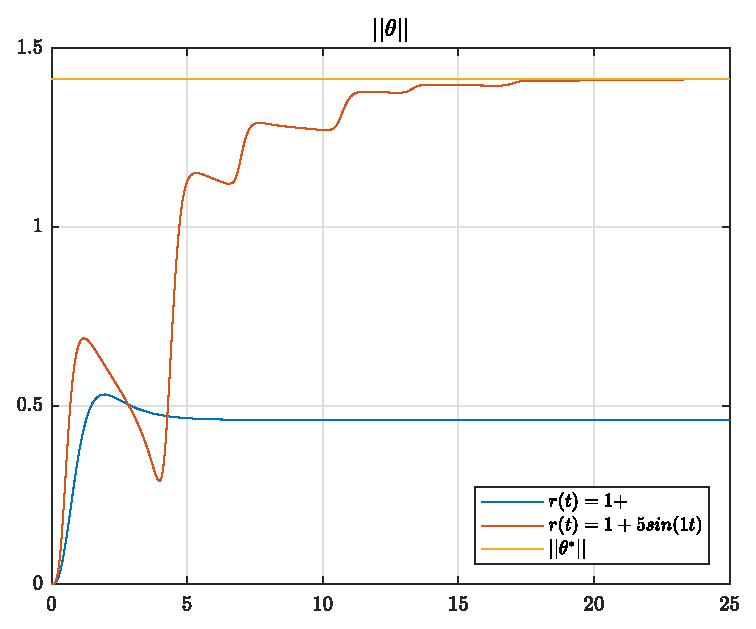
\includegraphics[width=12cm]{figs/gradiente/modtheta/sim01_r1r2.eps} \\[2mm]
\end{figure}

\begin{figure}[H]
  \centering
  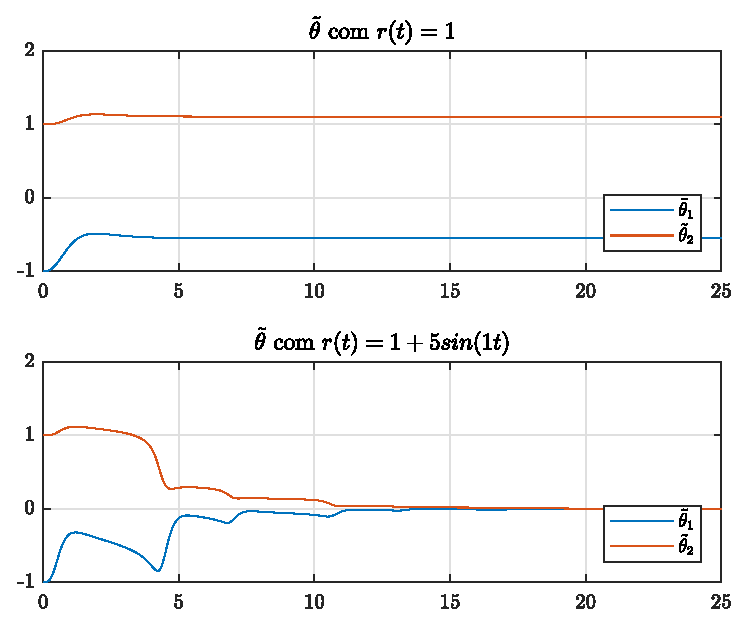
\includegraphics[width=12cm]{figs/gradiente/tiltheta/sim01_r1r2.eps} 
\end{figure}


\begin{figure}[H]
  \centering
  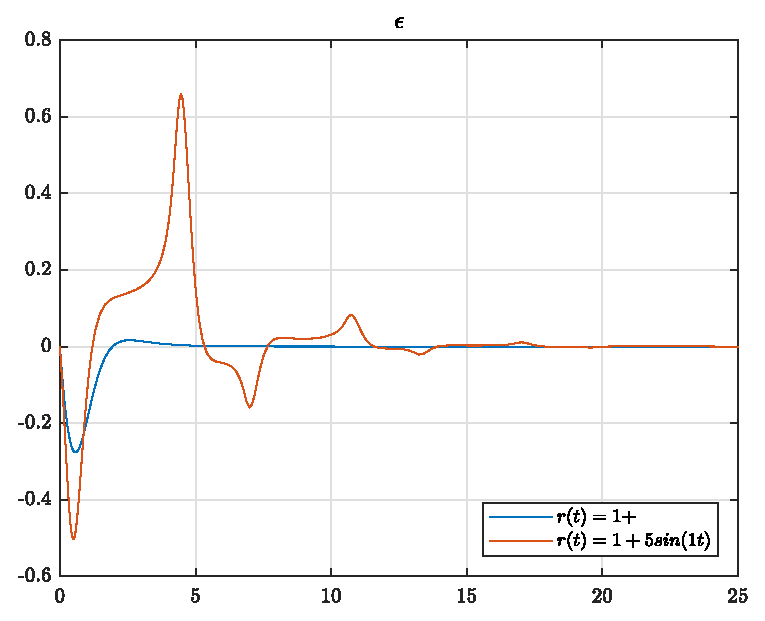
\includegraphics[width=12cm]{figs/gradiente/epsilon/sim01_r1r2.eps} 
\end{figure}

\newpage%

\begin{align*}
  y &= \frac{s+1}{s+4s+4}u\,,  &  \Lambda &= \frac{1}{s+2s+1}\,, & \theta(0) &=
  0\,,\\
  \gamma &= 10\,, & r &= \HI{$10\textrm{sin}(0.63493t)$} e
  \HI{$30\textrm{sin}(0.63493t)+25\textrm{sin}(4.5669t)$}\, \,.
\end{align*}

\bigskip%
\begin{figure}[H]
  \centering
  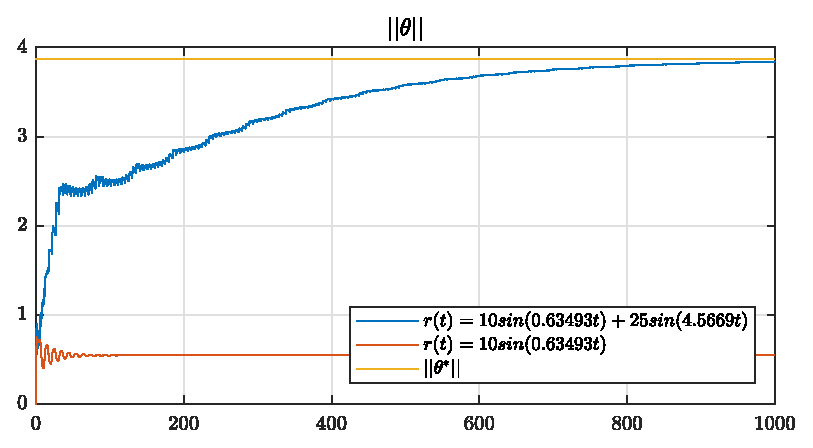
\includegraphics[width=12cm]{figs/gradiente/modtheta/sim02_r1r2.eps} \\[2mm]
\end{figure}

\begin{figure}[H]
  \centering
  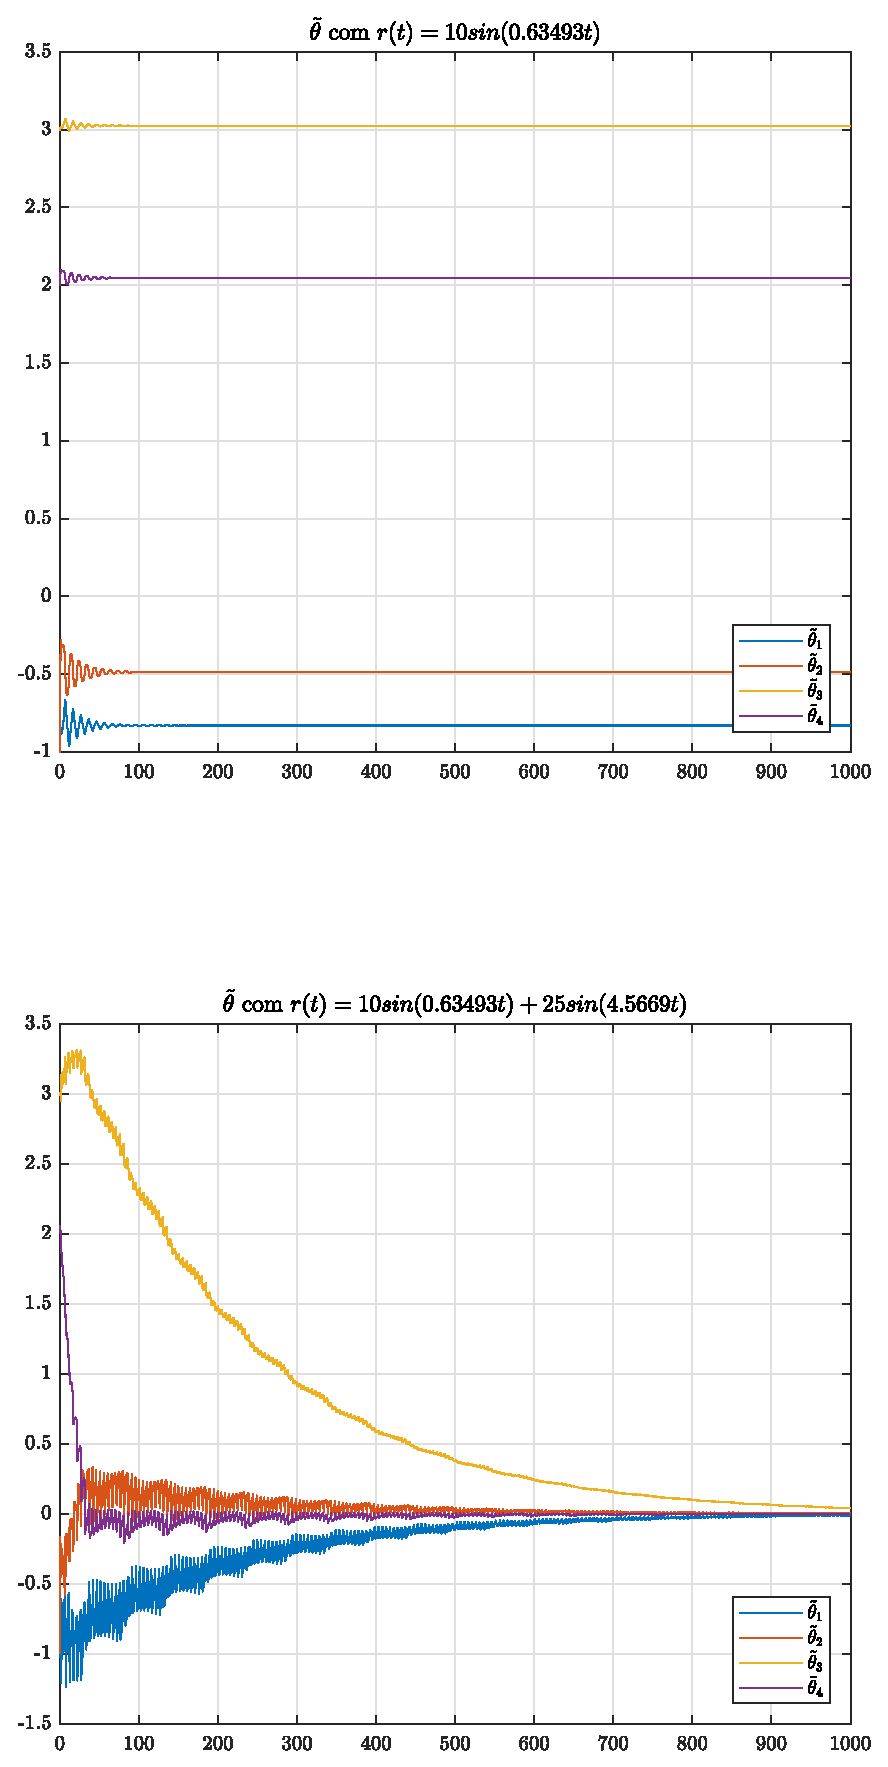
\includegraphics[width=12cm]{figs/gradiente/tiltheta/sim02_r1r2.eps} 
\end{figure}


\begin{figure}[H]
  \centering
  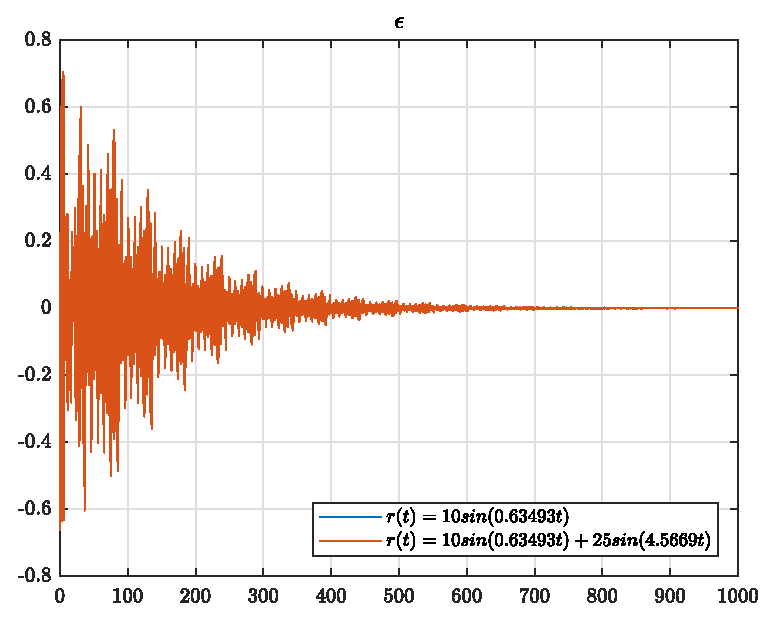
\includegraphics[width=12cm]{figs/gradiente/epsilon/sim02_r1r2.eps} 
\end{figure}
%---------------------------------------------------------------------
\subsection{Simula��o \#2}

Na segunda simula��o, observamos o comportamento do sistema para varia��es no p�lo do filtro.

%\bigskip%
%Par�metros e condi��es iniciais:
%
\begin{align*}
  a_p &= -2\,,  &  y_p(0) &= 0\,, & \theta(0) &= 0\,, \\
  a_m &= 1\,,   &  y_m(0) &= 0\,, & \gamma &= 5\,, \\
  r &= 1\,, & a_f &= \HI{3, 5}\,.
\end{align*}

\begin{figure}[H]
  \centering
  \includegraphics[width=12cm]{figs/e0/af3af5.eps} \\[2mm]
\end{figure}

\begin{figure}[H]
  \centering
  \includegraphics[width=12cm]{figs/epsilon/af3af5.eps} 
\end{figure}


\begin{figure}[H]
  \centering
  \includegraphics[width=12cm]{figs/theta/af3af5.eps} 
\end{figure}

\begin{figure}[H]
  \centering
  \includegraphics[width=12cm]{figs/yp/af3af5.eps} 
\end{figure}

\begin{figure}[H]
  \centering
  \includegraphics[width=12cm]{figs/u/af3af5.eps} 
\end{figure}

\newpage%
%---------------------------------------------------------------------
\subsection{Simula��o \#3}

Na terceira simula��o, observamos o comportamento do sistema para varia��es no p�lo desconhecido da planta.

%\bigskip%
%Par�metros e condi��es iniciais:
%
\begin{align*}
  a_p &= \HI{-2, -5}\,,  &  y_p(0) &= 0\,, & \theta(0) &= 0\,, \\
  a_m &= 1\,,   &  y_m(0) &= 0\,, & \gamma &= 5\,, \\
  r &= 1\,, & a_f &= 1\,.
\end{align*}

\begin{figure}[H]
  \centering
  \includegraphics[width=12cm]{figs/e0/ap-2ap-5.eps} \\[2mm]
\end{figure}

\begin{figure}[H]
  \centering
  \includegraphics[width=12cm]{figs/epsilon/ap-2ap-5.eps} 
\end{figure}


\begin{figure}[H]
  \centering
  \includegraphics[width=12cm]{figs/theta/ap-2ap-5.eps} 
\end{figure}

\begin{figure}[H]
  \centering
  \includegraphics[width=12cm]{figs/yp/ap-2ap-5.eps} 
\end{figure}

\begin{figure}[H]
  \centering
  \includegraphics[width=12cm]{figs/u/ap-2ap-5.eps} 
\end{figure}

\newpage%
%---------------------------------------------------------------------

\subsection{Simula��o \#4}

Na simula��o 4, variamos o p�lo do modelo de refer�ncia utilizado.

%\bigskip%
%Par�metros e condi��es iniciais:
%
\begin{align*}
  a_p &= -2\,,  &  y_p(0) &= 0\,, & \theta(0) &= 0\,, \\
  a_m &= \HI{2, 5}\,,   &  y_m(0) &= 0\,, & \gamma &= 5\,, \\
  r &= 1\,, & a_f &= 1\,.
\end{align*}

\begin{figure}[H]
  \centering
  \includegraphics[width=12cm]{figs/e0/am2am5.eps} \\[2mm]
\end{figure}

\begin{figure}[H]
  \centering
  \includegraphics[width=12cm]{figs/epsilon/am2am5.eps} 
\end{figure}


\begin{figure}[H]
  \centering
  \includegraphics[width=12cm]{figs/theta/am2am5.eps} 
\end{figure}

\begin{figure}[H]
  \centering
  \includegraphics[width=12cm]{figs/yp/am2am5.eps} 
\end{figure}

\begin{figure}[H]
  \centering
  \includegraphics[width=12cm]{figs/u/am2am5.eps} 
\end{figure}

\newpage%
%---------------------------------------------------------------------

\subsection{Simula��o \#5}

Por �ltimo, observamos o comportamento do sistema para varia��es nas condi��es iniciais da planta.

%\bigskip%
%Par�metros e condi��es iniciais:
%
\begin{align*}
  a_p &= -2\,,  &  y_p(0) &= \HI{0, 5}\,, & \theta(0) &= 0\,, \\
  a_m &= 1\,,   &  y_m(0) &= 0\,, & \gamma &= 5\,, \\
  r &= 1\,, & a_f &= 1\,.
\end{align*}

\begin{figure}[H]
  \centering
  \includegraphics[width=12cm]{figs/e0/yp00yp05.eps} \\[2mm]
\end{figure}

\begin{figure}[H]
  \centering
  \includegraphics[width=12cm]{figs/epsilon/yp00yp05.eps} 
\end{figure}


\begin{figure}[H]
  \centering
  \includegraphics[width=12cm]{figs/theta/yp00yp05.eps} 
\end{figure}

\begin{figure}[H]
  \centering
  \includegraphics[width=12cm]{figs/yp/yp00yp05.eps} 
\end{figure}

\begin{figure}[H]
  \centering
  \includegraphics[width=12cm]{figs/u/yp00yp05.eps} 
\end{figure}

\newpage%
%--------------------------------------------------------------------- \newpage
%---------------------------------------------------------------------
\section{Discuss�o}

A \textbf{simula��o \#1} mostra o comportamento do sistema para varia��es no sinal de refer�ncia. Como esperado e demonstrado na se��o 3.5 do livro \textit{Adaptive
Control Design and Analysis} de Gang Tao, a converg�ncia dos par�metros s� �
garantida quando o sinal de refer�ncia possui o mesmo n�mero de
frequ�ncias que o n�mero de par�metros desconhecidos (excita��es persistentes).

Na simula��o 1.1, o sistema � de primeira ordem com dois
par�metros desconhecidos. Logo, s�o necess�rias duas frequ�ncias diferentes no
sinal de refer�ncia para garantir que o erro de estima��o $\tilde{\theta}$
convirja para zero. Isso � verificado, j� que $\tilde{\theta}$ converge para
zero quando $r=1+5\textrm{sin}(t)$ (frequ�ncia em $\omega=0, \omega=1,
\omega=-1$) e n�o converge para zero quando o sinal possui apenas uma frequ�ncia
($r=1$). Um comportamento semelhante � verificado para os sistemas de segunda e
terceira ordens (simula��es 1.2 e 1.3, respectivamente). Vale observar que, em
todos os casos, $\epsilon = \tilde{\theta}^\intercal \phi$ converge para zero,
como � provado por Lyapunov.  Isso significa que, apesar de a estima��o dos
par�metros n�o ter garantia de converg�ncia para zero, os vetores $\tilde{\theta}$ e $\phi$ entram em quadratura, ou seja, ficam ortogonais.

A \textbf{simula��o \#2} mostra o comportamento do sistema para varia��es no
ganho de adapta��o $\Gamma$ para o m�todo do gradiente normalizado. Nesse caso, a varia��o da estima��o de par�metros � descrita pela f�rmula: $\dot{\theta}(t) = -\Gamma \, \phi(t) \, \epsilon(t) / m^2(t)$. Portanto, a varia��o � proporcional ao ganho de adapta��o, quanto maior o par�metro, mais r�pida ser� a estima��o. J� no caso do m�todo \textit{least-squares} normalizado, o valor inicial do ganho n�o impacta muito no regime transit�rio.

A \textbf{simula��o \#3} mostra o comportamento do sistema para varia��es nas condi��es iniciais. A rapidez da converg�ncia depende de qu�o pr�ximo os par�metros estimados est�o dos par�metros reais. Na simula��o 3.1, por exemplo, a converg�ncia � mais r�pida quando $\theta = \textbf{0}, \theta^* = \left[1 \, -1\right]$, por�m, na simula��o 3.3, ela � mais r�pida quando $\theta = \textbf{1}$, pois $\theta^* = \left[1 \, 1 \, 1 \, 0 \, 2 \, 2\right]$.

Observe que o comportamento dos sistemas � semelhante para ambos os m�todos
utilizados: \textit{Gradiente normalizado} e \textit{least-square
normalizado}. Pode ser provado que o m�todo \textit{Gradiente
normalizado} garante converg�ncia exponencial do erro para zero (Tao 3.5.2). J� o m�todo \textit{least-square normalizado} apenas garante converg�ncia, mas n�o
exponencial (Tao 3.5.3).

Tamb�m foi constatada, mas n�o relatada aqui, a interessante propriedade do m�todo \textit{least-square normalizado} em que $P^{-1} \, \tilde{\theta} = P_0^{-1} \, \tilde{\theta}(0) = \text{constante} \,$. 
%---------------------------------------------------------------------
%\bibliographystyle{agsm}
%\bibliography{bib,coe736}

%---------------------------------------------------------------------
\end{document}
